% !TeX root = ../diss.tex
In this chapter I describe how the DSL is implemented. Documentation for all publicly exposed functions can be found in appendix \ref{app:docs}.

\section{Repository Overview}
% TODO: include a file tree?
The majority of my code is in the \texttt{ppl} directory, which contains the core library, unit tests, statistical testing code and some example programs written using the library.

I have implemented my ppl as a library residing in the \texttt{lib} subdirectory, contained within the module \texttt{Ppl}. Opening this module in a script allows a user to use my library. Ppl includes several submodules, most importantly the \texttt{Dist} and \texttt{Inference} modules, which contains the code for representing, creating and combining distributions, and performing inference, respectively. These functions can be found in separate files in the inference folder, and are all exported in the inference module. The other modules exported in Ppl are plot, prim\_dist, and samples.

\texttt{Prim\_dist} contains code for using primitive distributions - as well as types which a user can provide to define their own distributions. It also defines functions which can be used by the user to create new primitive distributions.

The \texttt{Plot} module contains helper functions which wrap around Owl\_plplot, allowing users to easily create visualisations from distributions defined in my ppl. This includes histograms 

The \texttt{bin} directory contains several example programs to show how the ppl can be used to express many different models. 

The \texttt{test} directory contains basic unit tests as well as hypothesis tests to check the correctness of inference.

The \texttt{evaluation} directory contains code to compare my ppl to both hand-written inference procedures, as well as equivalent programs in other PPLs. There are several directories, which each correspond to a particular problem/model.

All code is written in OCaml 4.08, with the main dependencies being Jane Street's \texttt{Core} and \texttt{Owl} \cite{owl}.

\section{Language Design}
I chose to implement my language as a domain specific language (DSL) shallowly embedded into the main OCaml language. This allows models built in the ppl to be easily composed with other standard OCaml programs.

Using a shallow embedding means we can use all of the features of OCaml as normal, including branching (if/then/else), loops, references, let bindings, (higher-order) functions, and importantly, recursion. This can allow us to define models that do not terminate and are therefore invalid. However, we can write functions which are \textit{stochastic recursive} \cite{siegmund}, that is, functions which have a probability of termination that tends to 1 as the number of successive calls tends to infinity. This leads to functions which terminate their recursion non-deterministically. Any model which does not satisfy this will be considered an invalid model - unfortunately as it is not possible to determine whether or not a program will halt, this property cannot be enforced. 

I use a set of primitive distributions which can be combined (using arbitrarily complex deterministic OCaml code) to produce new more complex distribution. For example, one can take the sum of two discrete uniform distributions to simulate the addition of two dice rolls. 

PPLs in general are similar to normal programming languages, but need to support two extra operations - \texttt{sample} and \texttt{condition} \cite{gordon2014probabilistic}. The sample operator allows models to be built up .The condition operator has a few variants, which are covered in section \ref{sec:condition}.

\section{Representing Distributions}
In order to define my DSL, I needed data structures to represent probabilistic models as well as distributions that are used as both input and output. Input distributions are the primitive distributions that are used to build models and constrain observations. We have more information about these distributions, such as how to sample from them exactly and exact pdf functions, and this information is used in inference. The output of inference is usually a distribution which can be sampled from to obtain the posterior, but we generally want to also collate statistics about the posterior distribution. Since we only have an approximate sampler, we can output empirical distributions from which many statistics, e.g. mean, variance, cdf etc., can be approximated.

\subsection{Probability Monad}

As mentioned before, monads are a natural way to represent probability distributions. They allow the output from one distribution (essentially a sample), to be used as if it was of the type that the distribution is defined over. Essentially, the \texttt{bind} operation allows us to 'unwrap' the 'a dist type to allow us to manipulate a value of type 'a. We must then use \texttt{return} to `wrap' the value back into a value of type 'a dist. The type signature of bind is \texttt{'a m -> ('a -> 'b m) -> 'b m}, and return is \texttt{'a -> 'a m}, with m being the monad type.

Using monads also allows us to define several helper functions which can be used when working with distributions. For example, we can `lift' operators to the \texttt{dist} type, for example allowing us to define adding two distributions over integers or floats using liftM or liftM2. We can also fold lists of distributions using a similar technique.

Using monads also allows the use of the extended let operators introduced in OCaml 4.08. These allow the definition of custom let operators, which mimic do-notation in Haskell. This means that sampling from a distribution (within a model) can be done using the \texttt{let*} operator, and the variable that is bound to can be used as if it were a normal value. The one caveat is that the user must remember to \texttt{return} at the end of the model with whatever variable(s) they want to find the posterior over. The \texttt{and*} operator can also be used when we use several independent distributions in a row. This can make for more efficient sampling (and inference) since we have more information about the structure of the program. It is also a common pattern to set up a model by first independently drawing from several distributions. An example of let* and and* is given below.

% \begin{noindent}
\begin{ocamlcode-in}
let* x = normal 0. 1.
and* y = normal 0. 1. in
return (x + y)
\end{ocamlcode-in}
% \end{noindent}
		
I define my own functor for monads in order to define several helper functions. This functor takes a module wrapping any monad type and extends it with helper functions. The full module documentation for this can be found in appendix \ref{app:docs} (\texttt{Monad.Make\_extended}). An example if the liftM2 function, which allows normal operations to be lifted to distributions, e.g. an addition operator for the output for two distributions can be simply created by lifting the normal addition operator.

% \begin{noindent}
\begin{ocamlcode-in}
let ( +~ ) = liftM2 ( +. )
(* the distribution created by adding two normals *)
let d = (normal 0. 1.) +~ (normal 0. 1.)
\end{ocamlcode-in}
% \end{noindent}

However, there are many different underlying data structures which can be used to represent distributions. The simplest is a list of pairs representing a set of values and corresponding probabilities, \texttt{('a * float) list}. This is a very convenient and natural way to represent discrete distributions, with return and bind defined as in listing \ref{lst:monad_plist}. Here, \texttt{return} gives us the distribution with just one value, and bind combines a distribution with a function that takes every element from the initial distribution and applies a function that creates a set of new distributions. The new distributions are then `flattened' and normalised. This approach has been used to create functional probabilistic languages \cite{erwig}, but has several drawbacks, primarily the fact that it cannot be used to represent continuous distributions, and that inference is not efficient - there is no information from the model encoded in this representation, such as how random variables are combined or from what distributions they came from.


% TODO: finish the snippet, write unduplicate properly
\begin{listing}[!ht]
	\ocamlcode{code_snippets/probmonad_list.ml}	
	\caption{Simple Probability Monad}
	\label{lst:monad_plist}
\end{listing}

A major problem with this approach is that in flattening distributions, we must make sure that duplicated values are combined, and this approach is $O(n^2)$ when using a list since we must scan up to the length of the entire list for every element. A better option is to use a map, which is provided in Core, and implemented as a balanced tree, significantly improving the time complexity of combining distributions.

\begin{listing}[!ht]
	\ocamlcode{code_snippets/probmonad_map.ml}	
	\caption{Simple probability monad using a map}
	\label{lst:monad_pmap}
\end{listing}

Although this is not the final data structure I chose for general probabilistic models, it is the one I used for discrete empirical distributions.

\subsection{GADT} \label{sec:gadt}
% TODO: check this
The structure that I landed on to represent general models is a generalised algebraic data type. GADTs are often used to implement interpreters in functional languages, and have been used to represent probabilistic models. The GADT I implement here (and some inference algorithms) is based on (Scibior et al. 2015)\cite{scibior2015practical}. This represents a model in a very general way, and can then be `interpreted' by a sampler or an inference algorithm. For sampling, I traverse the model, ignoring conditionals to enable forward sampling from the prior. For inference, I provide some inference functions as transforming the conditional distributions to distributions without any conditional statements, allowing sampling to be performed as normal. Some inference functions are also implemented by generating an empirical distribution that can be sampled from similarly. Primitive distributions also have a special variant (which takes a different \texttt{primitive} type). We can find the exact pdf/cdf of these distributions, unlike the \texttt{dist} type, which can only be sampled from. Listing \ref{lst:gadt1} shows each of the variants. The monad functions are also provided, which construct the corresponding variant in the GADT. \texttt{Return} represents a distribution with only one value, and \texttt{Bind} contains a distribution and a function, which represents that function being applied to the output from that distribution.

\begin{listing}[!ht]
	\ocamlcode{code_snippets/gadt.ml}	
	\caption{Representing a probabilistic model using a GADT}
	\label{lst:gadt1}
\end{listing}

An important feature of this type is that it is polymorphic - this allows distributions to be defined over any type. Usually, this type is floats or integers, but this allows us to define distributions over anything, including distributions - a feature used in certain models such as a Dirichlet process.

\subsection{Primitive Distributions}
In PPLs, users build complex models by composing more simple elementary primitive distributions (ERP) \cite{pmlr-v15-wingate11a}. These primitive distributions need to have a few operations defined on them, namely \texttt{sample, pdf, cdf} and \texttt{support}.

An extension goal achieved here is to allow users to define their own primitive distributions if they have not already been defined in the library. A concrete use case - I have not implemented the Poisson distribution as a primitive distribution, but you can imagine models which need to use the Poisson as a building block. To achieve this, the user simply has to write a function which takes the parameters of the distribution as arguments and return a first class module matching the primitive distribution signature. This technique also allows users to use modules that they may have already defined, and constrain them to the required signature for use in the PPL.

The type of a primitive distribution is \texttt{type 'a prim\_dist = (module PRIM\_DIST with type t='a)}, with the \texttt{PRIM\_DIST} signature defined as in listing \ref{lst:prim-sig}. 

% TODO: put these side by side instead
\begin{listing}[!ht]
	\ocamlcode{code_snippets/prim_sig.ml}	
	\caption{Signature of the module that primitive distributions must implement}
	\label{lst:prim-sig}
\end{listing}

An example of this being used to add a new primitive distribution is given in listing \ref{lst:new-dist}, for the specific case of the Poisson distribution. The \texttt{Poisson} distribution can be used as other primitives are, e.g. in \texttt{observe} statements.

\begin{listing}[!ht]
	\ocamlcode{code_snippets/new_dist.ml}	
	\caption{Adding a new distribution as a primitive}
	\label{lst:new-dist}
\end{listing}

\subsection{Empirical Distributions}

The output of Bayesian inference is a probability distribution over the variable we are concerned with. Ideally, we would be able to produce an exact posterior distribution, and be able to extract exact statistics from it. However, approximate inference only allows us to create functions to sample from this posterior. We can define a signature for a type of an empirical distribution that is created from posterior distributions and can be used to calculate useful properties such as the pdf or cdf. The type is abstract to allow different implementations for discrete and continuous distributions. For discrete distributions, I use a \texttt{Core.Map}\footnote{\url{https://ocaml.janestreet.com/ocaml-core/latest/doc/base/Base/Map/index.html}}. Continuous distributions use a dynamically resizing array - adding each sample is then $O(1)$ amortized, and statistics can be calculated using Owl's functions that operate on arrays. A constraint on continuous distributions of this type is that they are defined over floats, and only represent one dimension.
% Creating values with these types required passing a first class module representing the type of the keys - this is so that an appropriate compare function can be used in the internal tree data structure.

% I also provide modules which are backed by the polymorphic versions of these data structures (\texttt{Core.Map.Poly}). These types don't require the use of first class modules to create objects, since the keys are compared using the polymorphic compare function. While this makes using the module simpler to use (no need to pass the first class module), it also makes them more inefficient due to the use of polymorphic comparison.

\begin{listing}[ht]
	\ocamlcode{code_snippets/empirical_sig.ml}
	\caption{Signature for empirical distributions}
	\label{lst:empirical}
\end{listing}

The signature given in listing \ref{lst:empirical} is implemented for both continuous and discrete distributions. For the continuous case, I perform binning to approximate the continuous distribution by a discrete one - exemplified by figure \ref{fig:binning} - in order to approximate the pdf. The number of bins used is calculated automatically from the number of samples taken.

\begin{figure}[!hb]
	\centering
	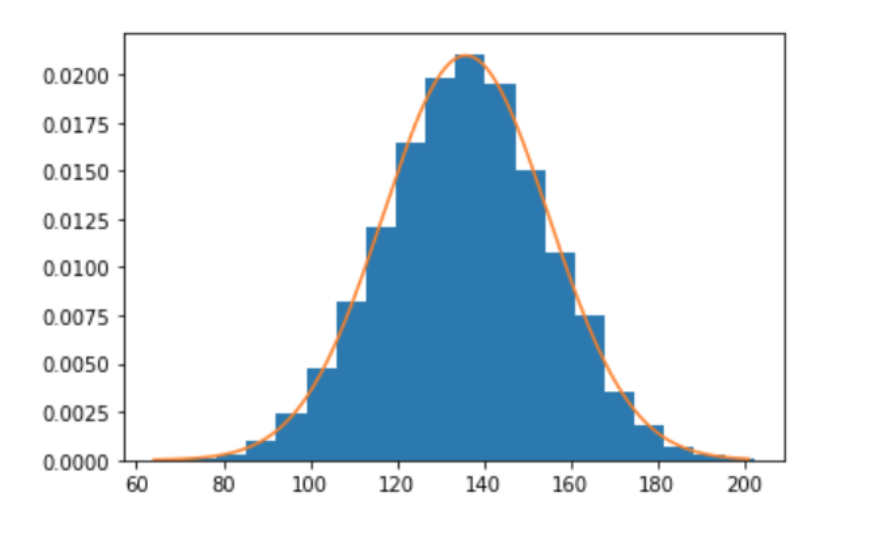
\includegraphics[width=\textwidth]{figs/bins.png}
	\caption{An example of approximating a continuous distribution using discrete bins}
	\label{fig:binning}
\end{figure}

\section{Conditioning} \label{sec:condition}

The GADT described in section \ref{sec:gadt} can be used to describe general models, in particular conditional distributions, thanks to the \texttt{Conditional} variant. Without this variant, we can only define prior distributions, but including it means we can incorporate observed data into our models and perform inference.

% https://www.robots.ox.ac.uk/~twgr/assets/pdf/rainforth2017thesis.pdf - section on conditioning, pg.42
The condition variant in my GADT is used to assign scores to traces, and takes a function which takes an element and returns a float, a `score'. This score represents how likely the current trace is, given the value passed to the functions. In this way, we can represent observations.
	
I have also implemented a few helpers to make it easier to condition models. The three main helpers are \texttt{condition}, \texttt{score} and \texttt{observe}, which are all specific cases of the general \texttt{Condition} variant. 
	
The \texttt{condition} operator is used for hard conditioning, which conditions the model on an observation being true. If true is passed in, then the score assigned is 1, and if false, the score assigned is 0. This score represents how likely it is for the current trace to occur, and different inference algorithms will use this information to produce a distribution over all possible traces. We can use this operator to constrain certain variables or outcomes in a model. For example in the below model, we roll two dice and observe that the sum is 4 - we can then find the distribution over the first die (which won't include 4,5 or 6 since they are >=4, the sum).
	
% TODO: put this inline minted (not file) 
% Also not a huge box
\ocamlcode{code_snippets/dice_sum.ml}	
		
This function is mostly useful for discrete models when using equality in this manner, since the probability of observing any given value in a continuous distribution is zero. However, if we are dealing with ranges, then we can use hard conditioning as in the model below, which constrains the standard normal distribution to be positive.
	
% TODO: put this inline minted (not file) 
% Also not a huge box
\ocamlcode{code_snippets/half_normal.ml}

For soft conditioning, for example an observation that we know comes from a certain distribution, there is an \texttt{observe} function. This function is essential for continuous distributions, since the probability of observing any one value is 0, making hard conditioning since it will just reject every trace. Instead, we can use the pdf function of the distribution to determine how likely that observation is in the model.
	
The \texttt{score} function is similar to the condition operator, except instead of 0, it assigns a particular constant score (any float) to the trace. This is generally used in a branch, where a constant score will be assigned depending on some (deterministic) condition.

% \begin{noindent}
\begin{listing}[!htb]
	\centering
\begin{ocamlcode-in}
let condition b d = Conditional((fun _ -> if b then 1. else 0.), d)
let score s d = Conditional((fun _ -> s),d)
let observe x dst d = Conditional((fun _ -> Primitive.pdf dst x),d) 
\end{ocamlcode-in}	
	\caption{The definitions of the different conditioning operators}
	\label{lst:cond}
\end{listing}
% \end{noindent}

\section{Forward Sampling}
% https://www.robots.ox.ac.uk/~twgr/assets/pdf/rainforth2017thesis.pdf - sec 7.1, pg 135
The simplest operation to define on models is to sample from them. Sampling from conditional distributions required inference, and is discussed in section \ref{sec:inference}. Here, we run a probabilistic program 'forwards', that is, running a generative model and seeing the outputs without conditioning on observed data.
	
In PPLs, a complete program can be thought of as a posterior, $P(\theta\mid x)$, the distribution of a parameter given some observed data. The generative model, i.e. the program without condition statements, can be thought of as the prior distribution, $P(\theta)$. The condition statements then define the likelihood model, that is, $P(x\mid \theta)$, the probability of the observations in the current model (the prior). So finding the prior is the same as disregarding the conditionals (essentially ignoring the data). Sampling is only difficult in the presence of conditionals (as this requires inference), so this allows us to sample from the prior using the same sample function defined before. We can also transform any \texttt{'a dist} into a different \texttt{'a dist} that is the prior by ignoring conditional statements.
	
We can also take into account the conditionals, and produce weighted samples, with the weight being the score assigned by each conditional branch, accumulated by multiplying all the scores. This gives us a set of values with corresponding weights which represent how likely those values are. An important property of these weights is that they are not normalised, so we cannot use this to find the posterior directly. I have implemented several variants of functions for finding the prior and sampling, all with the same concept as below.

% TODO split into two panes
\ocamlcode{code_snippets/prior_sample.ml}

The function for generating a prior does not directly take samples, but manipulates the structure of the dist GADT. For example, in the \texttt{Bind} branch, it actually introduces 2 new bind variants (via \texttt{let*}) which produces a new distribution lazily. This makes it easier to use the prior within inference algorithms, and allows it to be composed with other distribution modifying functions.

\section{Inference} \label{sec:inference}

Inference is the key motivation behind probabilistic programming. Up to this section, we have discussed how to represent models but not do anything with them that couldn't be done in a standard language. With inference, we can produce a sampler which will accurately reflect a posterior distribution.

Inference can be thought of as a program transformation \cite{scibior2015practical} \cite{Zinkov2016ComposingIA}. In my ppl, this corresponds to a function of type \texttt{'a dist -> 'a dist}. This method allows for the composition of inference algorithms, exemplified in section \ref{sec:pimh}.

% use equations from here: https://arxiv.org/pdf/1507.00996.pdf
	
% Since I have used a trace-based approach, we can characterise the posterior probability of a trace as (from the previous chapter):
% % https://www.robots.ox.ac.uk/~twgr/assets/pdf/rainforth2017thesis.pdf - pg.52
% $$p(x_{1:N}|y_{1:N})\propto\tilde{p}(y_{1:N},x_{1:N})$$
	
% We can now see how this formula corresponds to a program in my ppl. The example below is a very simple model, which adds two numbers drawn from discrete distributions, and observes a value.
	
% TODO: write example program, and relate to terms in formula
	
\subsection{Enumeration} \label{sec:enum}
Enumeration is the simplest way to perform exact inference on probabilistic programs, and essentially consists of computing the joint distribution over all the random variables in the model. This involves enumerating every execution path in the model, in this case performing a depth first search over the \texttt{dist} data structure. For every \texttt{bind} (i.e. every \texttt{let*}), there is a distribution ($d$) and a function from samples to new distributions ($f$). I call this function on every value in the support of the distribution $d$, and then enumerate all the possibilities. The final output is a \texttt{('a * float) list}, from which duplicates are removed and is then normalised, so that the probabilities sum to one.
	
\begin{listing}[ht]
	\ocamlcode{code_snippets/enumerate.ml}
	\caption{Enumerating all paths through a model}
	\label{lst:enum}
\end{listing}
	
This method is very naive, and therefore inefficient. Since we essentially take every possible execution trace, we do not exploit structure such as overlapping traces. This can be made slightly more efficient by using algorithms such as belief propagation \cite{belief-prop}, but they still only work on models made up from discrete distributions (and are not compatible with the way I represent models). Exact inference of this kind only works on models that can be represented as finite networks, and exact inference for Bayesian networks is in fact NP-hard\cite{cooper1990computational}. So instead, most of my project focuses on approximate inference.
	
\subsection{Rejection Sampling} \label{sec:rej}
% https://www.cs.ubc.ca/~schmidtm/Courses/540-W18/wood.pdf pg30
% Ancestral sampling, very good explanation of rejection
% Why rejection doesn't work for continuous, so must use importance instead -->
% http://www.cs.tut.fi/~elomaa/teach/AI-2013-9.pdf
% Hard rejection
In my implementation of rejection sampling, we take samples from the prior, with accumulated scores. If the score is above some constant threshold, then we accept the sample, and if not, we reject the sample. The specific case of the general rejection sampling algorithm we use here sets the proposal distribution as the prior, and we use the scores to approximate the density function of the posterior. The implementation is shown in listing \ref{lst:rej}.
% todo: code of rejection sampling

\begin{listing}[!htb]
	\centering
	\ocamlcode{code_snippets/rej.ml}
	\caption{Simplest rejection sampling method}
	\label{lst:rej}
\end{listing}

This method is naive, since it runs an entire trace even if the first condition dropped the score below the threshold. An optimisation I implemented is to short-circuit this, and reject as soon as the trace goes below the threshold. This does slightly increase the time taken for small models, and so is not the default. It is also implemented as a dist transformation, so can again be used with the same sample methods.

This particular function is hard rejection, since samples with a lower score are always rejected. I have also implemented functionality to perform `soft' rejection. This method instead sets the probability of acceptance being the score attached to the sample.

A problem with rejection sampling is if conditions make most execution traces very unlikely. This means it will take a very large number of samples to have enough (or any) accepted samples. An example is given in listing \ref{lst:bad-reject}, where the condition only has a 1\% chance of being true. This means that, on average, for every 1000 samples, we will only accept one.

% \begin{noindent}
\begin{listing}[!htb]
	\centering
	\begin{ocamlcode-in}
let* x = bernoulli 0.001 in
condition (x=0)
(return x)
	\end{ocamlcode-in}
	
	\caption{An example of a model that is very inefficient under rejection sampling}
	\label{lst:bad-reject}
\end{listing}
% \end{noindent}
% 
\subsection{Likelihood Weighting} \label{sec:likelihood-wighting}
% http://www.cs.tut.fi/~elomaa/teach/AI-2013-9.pdf
	
Likelihood weighting is an importance sampling method, when the proposal distribution we use is the prior. We want any algorithm we use to be as general as possible, and not need to be tuned using auxiliary distributions chosen by hand. Since for any model we can find the prior distribution easily, it is natural to use this as a proposal distribution here - this can be seen in several of the implementations of inference. 

The implementation of likelihood weighting is simple - we simply take a set of samples (with weights) from the prior, remove duplicates and normalise, and use this set of particles as a the categorical distribution representing the posterior.
% \begin{noindent}	
\begin{listing}[!htb]
	\centering
	\begin{ocamlcode-in}
let importance n d = 
  let particles_dist = sequence @@ List.init n ~f:(fun _ -> prior d) in
  let* particles = particles_dist in 
  categorical particles
	\end{ocamlcode-in}
	\caption{Likelihood weighting}
	\label{lst:imp}
\end{listing}
% \end{noindent}

The sequence function is a monad function that takes a list of distributions and fold them together so that they act as a single distribution returning entire lists. This allows The use of \texttt{(let*)} to sample a set of particles at once, and use them directly as the distribution.
% code of importance sampling.

\subsection{Metropolis Hastings} \label{sec:mh}
Metropolis Hastings is an MCMC algorithm, and so is used to find a Markov chain with the stationary distribution equal to the target distribution, here the posterior. There are many variants of this algorithm, and the one I implement here is the independent metropolis hastings (IMH) algorithm. I use the prior as a proposal distribution, using scores as an approximation to a density function. The algorithm is outlined below.
\begin{itemize}
	\item Let $\pi$ be the target distribution that we want to sample from.
	\item Let $q$ be the density function of the prior, approximated by the scores.
	\item Initialise by taking a sample from the prior as the first state in the chain.
	\item Let x be a sample from the prior.
	\item Let y be the last state in the chain.
	\item Calculate the acceptance probability, $\alpha(x,y)$ by \eqref{eq:accept}
	      \begin{equation}
	      	\label{eq:accept}
	      	\alpha(x,y) = 
	      	\begin{cases}	
	      		\min{\left( \frac{\pi(y)q(x)}{\pi{x}q(y)},1 \right) } & \pi(x)q(x) > 0 \\
	      		1                                                     & \pi(x)q(x) = 0 \\
	      	\end{cases}
	      \end{equation}	      	      	      	      
	\item The state x is then accepted with probability $\alpha(x,y)$. If accepted, we use x as the next state, or if rejected, we re-use y as the next state. 
\end{itemize}

This produces a Markov chain with transition probability: \[p(x, y) = q(y)\alpha(x, y) \quad\quad y\neq x\].
It is known as `independent' metropolis hastings since subsequent candidate states ($x$) are independent on previous values of states.

% https://probmods.org/chapters/inference-algorithms.html
% MCMC section
I have implemented IMH as a function transforming \texttt{'a dist}s (\texttt{'a dist -> 'a dist}). This allows it to be composed with other inference algorithms, as well as allowing the standard sample function to be used on the output. To model a Markov chain, I use a \texttt{Core.Sequence}, which is a data structure for a lazy list. The creator function uses a function that takes a previous state to produce a new state and output a value - analogous to the transition function. In this case, the output is the same as the state.

One important property of the return distribution is that consecutive sample statements will need to return different values (to simulate running the chain). In order to achieve this, I create some mutable state - the sequence, which will take a step every time sample is called on the output distribution. In order to make sure this sequence is persistent, I use a reference and put it after a bind (let*) statement, incrementing the chain every time the function is called (which is only on sampling). Since the bind statement contains a function, the reference is closed over and is persistent to the output distribution.

\begin{listing}[!htb]
	\centering
	\ocamlcode{code_snippets/mh.ml}
	\caption{Metropolis hastings}
	\label{lst:mh}
\end{listing}

\subsection{Bootstrap Particle Filter} \label{sec:pf}
% https://probmods.org/chapters/inference-algorithms.html
% particle filter section
Particle Filters are a class of algorithms which use particles to approximate a posterior. This is similar to the technique I used in importance sampling (\ref{sec:likelihood-wighting}), but the difference here is that the particles are sequentially updated as we observe condition statements (i.e. as we observe data). In fact, an example of a particle filtering algorithm is sequential importance sampling, but here I use an algorithm called the bootstrap filter\cite{particlefilter}.

The code given in listing \ref{lst:smc} transforms a conditional distribution to a new conditional distribution. In order to find the posterior, we simply ignore the conditional by finding the prior after using the smc method.

\begin{listing}[!htb]
	\centering
	\ocamlcode{code_snippets/smc.ml}
	\caption{Particle Filter}
	\label{lst:smc}
\end{listing}

The GADT is traversed top down, with particles being initialised at a `leaf' - primitives or returns. From this root, bind functions apply functions to the particles, and conditional statements updates the weights and resamples. The \texttt{resample} function takes a set of particles and takes samples from this set with replacement - this is the `bootstrap' resampling method. The output distribution is conditioned by the total weight of all particles.

Increasing the number of particles finds a more accurate distribution, but also increases the amount of time and memory required.

\subsection{Particle Cascade} \label{sec:pc}
The particle cascade algorithm (also Asynchronous Sequential Monte-Carlo) is an algorithm that extends the particle filter, introduced in (Paige et al. 2014)\cite{paige2014asynchronous}. It uses a lazily generated infinite set of particles, which allows it to be `anytime', that is, it can generate more particles without having to start regenerate a large particle set from scratch. It also features a parallelisable re-sample step, although I will not make use of this feature, since I am not using multi-core OCaml.

The main implementation difference is that instead of resampling, a particle `branching' operation is used, which produces a lazily generated set of particles at each resample step. Each particle produces 0 or more children to be used in the next iteration.

\subsection{Particle-Independent Metropolis-Hastings} \label{sec:pimh}

SMC and MCMC algorithms are two distinct classes of algorithms, but can be combined to produce more efficient inference procedures. A simple example of these algorithms (known as PMCMC), is the particle-independent metropolis-hastings algorithm\cite{pmcmc}. This algorithm first uses a particle filter to find an approximation of the posterior, then uses this approximation as a prior distribution for metropolis-hastings.

% TODO: describe maths using https://www.maths.lancs.ac.uk/~sherlocc/CompStats/Dawn_of_Time/PseudoMarg/compstats_PIMH_BT.pdf

Due to the fact that my PPL allows composition of inference algorithms, a basic implementation is very simple.

% \begin{noindent}
\begin{ocamlcode-in}
let pimh k n d = mh k (Smc.smc n d)
\end{ocamlcode-in}
% \end{noindent}
However, there are flaws in this implementation, since any sampler produced is slow and can be made more efficient.
In addition, the reason this works is because the \texttt{smc} function produces a dist with conditionals, which no other inference method does.

% These examples should really be in evaluation
\section{Visualisations}
Visualising the output distributions from inference can be done using the \texttt{Owl\_plplot} module, which allows plotting directly from OCaml, rather than having to interface with other programs manually. I have implemented several helper functions which simplify visualising distributions created by my PPL. Empirical distributions are approximated by histograms displayed as bar charts using \texttt{Owl\_plplot}.

For discrete distributions, this conversion is simple - each bar is simply the pmf (probability mass function) of the distribution at each value in the support. This is calculated by drawing $N$ samples, then for each value $x_i$, finding $\frac{n}{N}$, where $n$ is the number of samples that equal $x_i$, to find the approximate probability of that value in the distribution, $P(X = x_i)$.

Where there is an ordering on the type, discrete distributions can also have their cdf visualised. The cdf of a discrete distribution is a step function. The ordering is given by a first class module representing the type. There are cases where there is no natural ordering - for example a distribution over an arbitrary ADT, so this also allows a user to custom define the ordering.
% 
\begin{figure}[!htb]
	\centering
	\subfloat[PDF]{{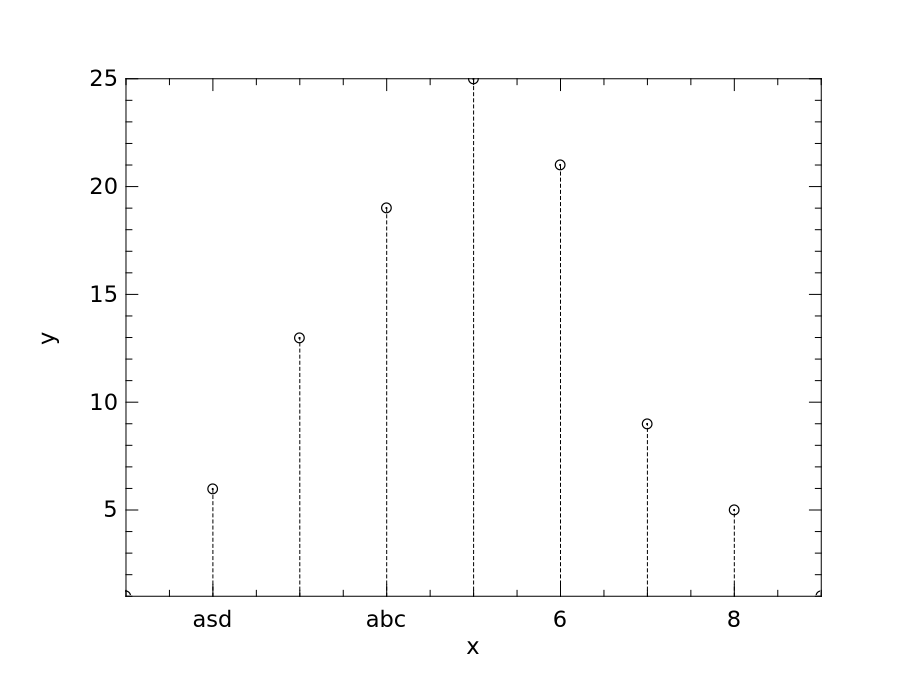
\includegraphics[width=0.4\textwidth]{figs/binompdf_hist.png} }}%
	\qquad
	\subfloat[CDF]{{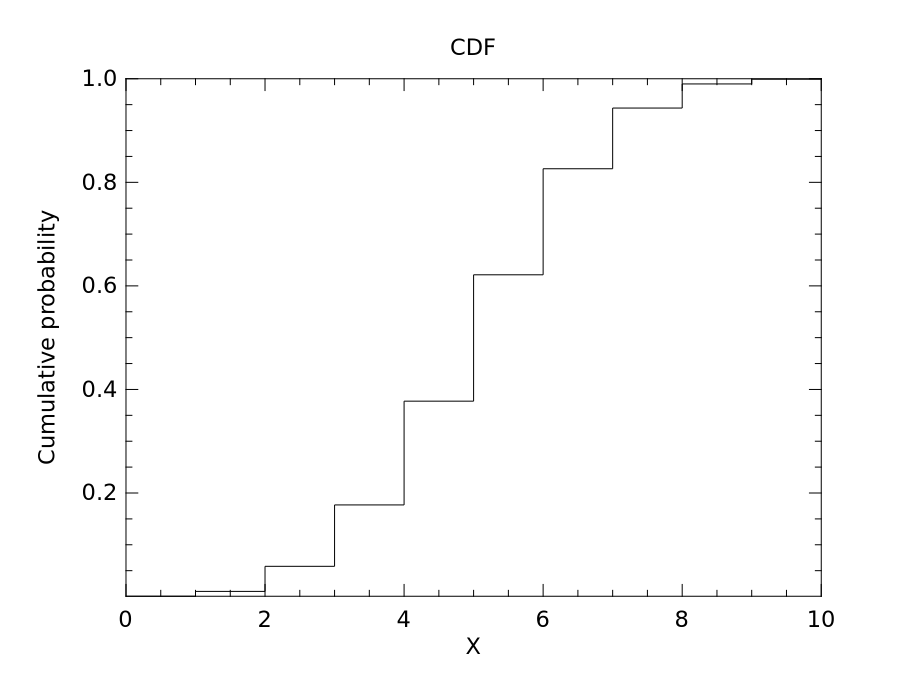
\includegraphics[width=0.4\textwidth]{figs/binom_ecdf.png} }}%
	\caption{Samples from a binomial distribution visualised}
	\label{fig:vis-binom}
\end{figure}
% 
Continuous distributions are also displayed as histograms, with a set of samples being put into $n$ equal width bins. The height of each bar is the the pdf (continuous analogue to the pmf), which is calculated by finding the number of samples in each bin, then dividing by the total number of samples. To display the cdf, we can display the empirical cdf directly as a scatter plot, or join points to draw a step function.

\begin{figure}[!htb]
	\centering
	\subfloat[PDF]{{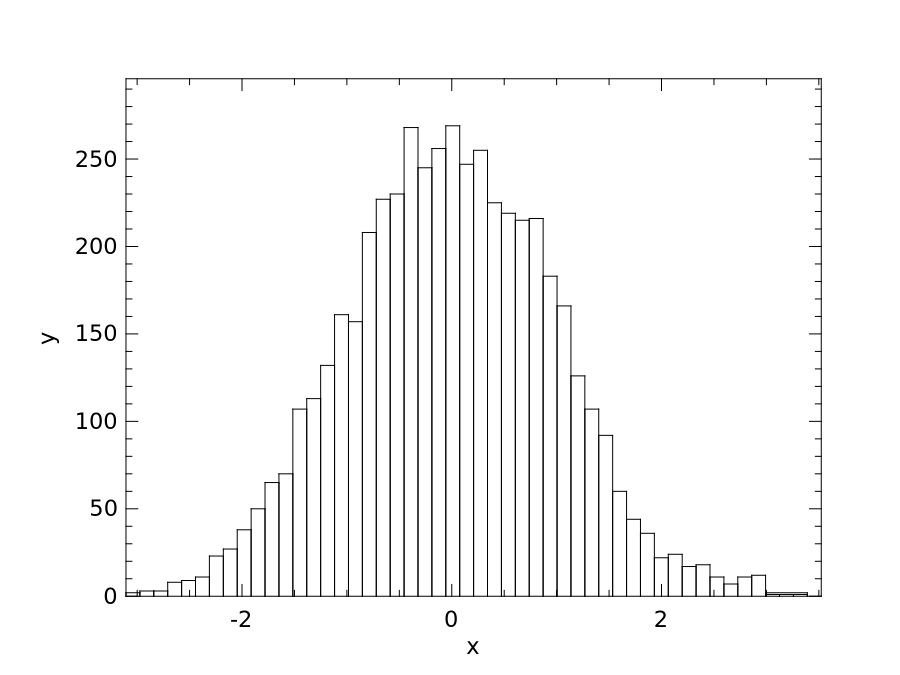
\includegraphics[width=0.4\textwidth]{figs/normpdf_hist.png} }}%
	\qquad
	\subfloat[CDF]{{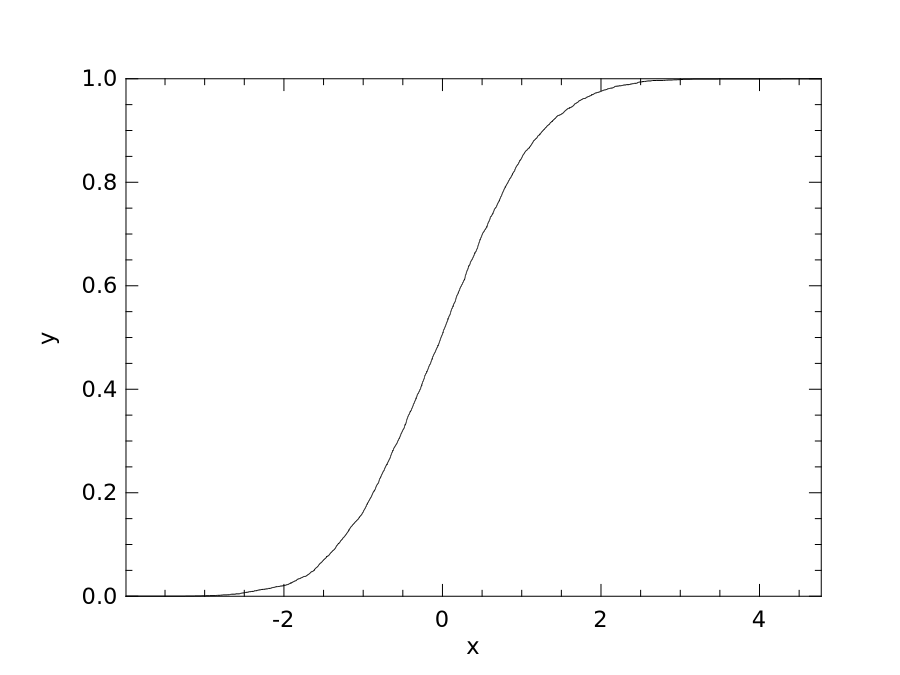
\includegraphics[width=0.4\textwidth]{figs/norm_ecdf.png} }}%
	\caption{Approximate pdf and cdf of samples from a standard normal distribution}
	\label{fig:vis-norm}
\end{figure}

Other important visualisations for continuous distributions are the Q-Q and P-P plots. These provides a way to qualitatively compare distributions. Q-Q plots plot the quantiles of two distributions against each other as a scatter plot - if all the points lie on the the line $y=x$, the distributions are identical. P-P plots plot the cdfs of two distributions against each other, that is, for two cdfs $F$ and $G$, the points (F(z), G(z)) are plotted for some values of z in the range $(-\infty,+\infty)$. Both these plots are often used to find the differences between some theoretical expected distribution and the distribution given by some data. This can be used in the PPL context to find whether a distribution given by a model matches what was expected in the theory. Figure \ref{fig:vis-qq} shows the output of inference for a model that is expected to output a beta distributions (the coin model in section \ref{sec:coin}) - the points are close to the expected line, visualising a successful inference procedure.

\begin{figure}[!htb]
	\centering			
	\subfloat[Q-Q plot]{{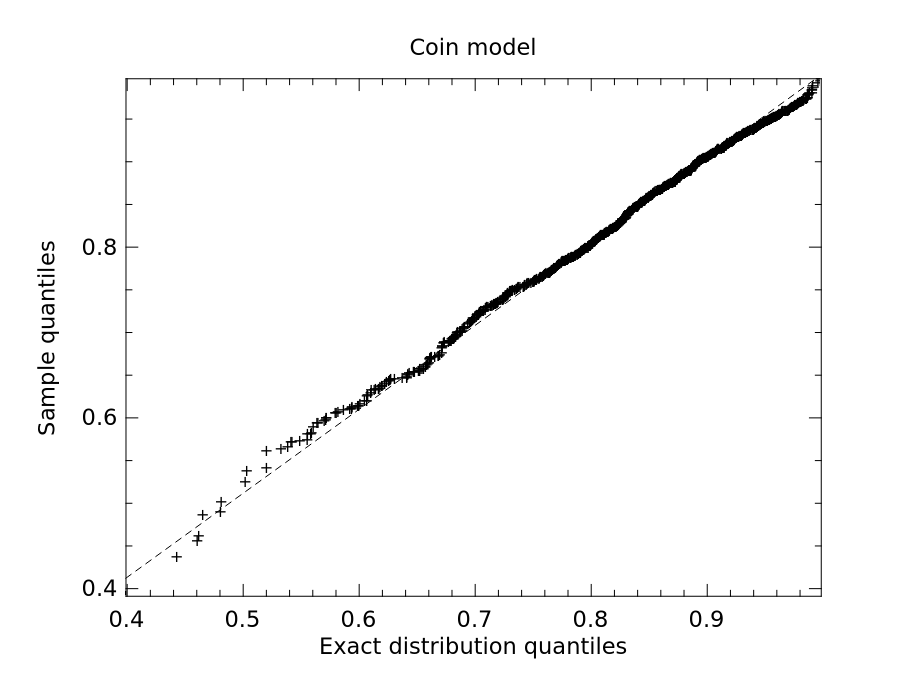
\includegraphics[width=0.4\textwidth]{figs/qq.png} }}%
	\qquad
	\subfloat[P-P plot]{{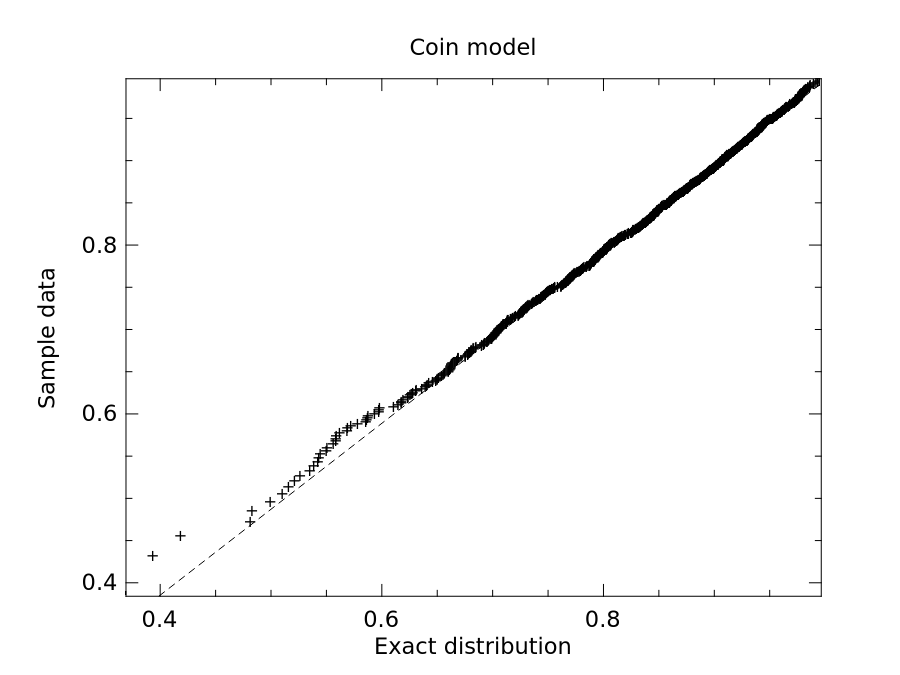
\includegraphics[width=0.4\textwidth]{figs/pp.png} }}%
	\caption{Plots to compare inferred distributions with the exact solutions}
	\label{fig:vis-qq}
\end{figure}

For primitive continuous distributions, a smooth line can also be drawn since we have a function that can calculate the exact pdf or cdf. This can also be overlaid onto a histogram, to again compare two distributions. Figure \ref{fig:vis-samples} shows an exact beta distribution overlaid onto samples taken from a beta distribution.

\begin{figure}[!htb]
	\centering
	% \subfloat[Code that generated the plot]{{\inputminted{ocaml}{code_snippets/plotter.ml} }}%
	% \qquad
	% \subfloat[P-P plot]{{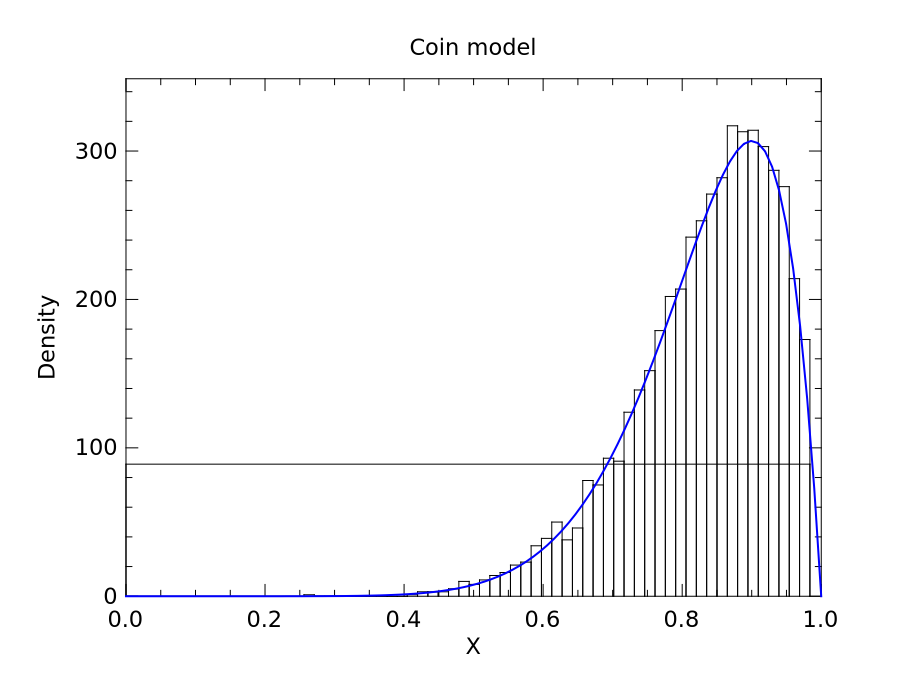
\includegraphics[width=0.4\textwidth]{figs/coin_compare.png} }}%
																											
	\begin{minipage}{0.45\textwidth}
		\centering
		\inputminted{ocaml}{code_snippets/plotter.ml}	
		\captionof{listing}{Code to produce plot}
	\end{minipage}
	\begin{minipage}{0.45\textwidth}
		\centering
		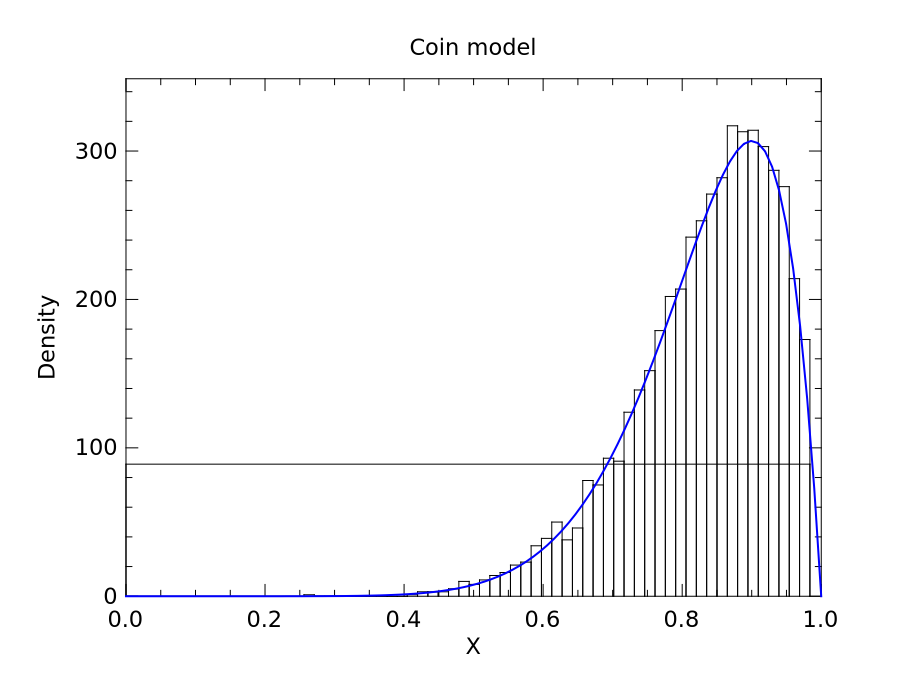
\includegraphics[width=\linewidth]{figs/coin_compare.png}
		\captionof{figure}{Output}
	\end{minipage}
																											
	\caption{The approximate and exact pdf of the output of inference for a biased coin model}
	\label{fig:vis-samples}
\end{figure}


\section{Testing}

Automated testing of PPLs is difficult for reasons outlines in the preparation. However, I still wrote basic unit tests. The test framework I used, Alcotest, lets me check that outputs of functions match expected values. This allows me to test all deterministic helper functions, e.g. normalise. It also lets me test the exact inference method, and very simple distributions and models which only contain a single value. I also used an additional library Quickcheck, to test that a specified invariant holds for a function - it uses randomly generated inputs to check the widest range of values. As an example, for the normalise functionwe expect that the output probabilities always sum to one, no matter the input array - the test is given below.

% \begin{noindent}
\begin{ocamlcode-in}
let test_normalise_sum_to_1 =
QCheck.Test.make ~count:1000 ~name:"test normalisation"
QCheck.(list (pair int float)) (fun l ->
((List.sum (module Float) ~f:snd @@ normalise l)) = 1.)
\end{ocamlcode-in}
% \end{noindent}

The test output and code coverage output can be seen in figure \ref{fig:test-out}.
\begin{figure}[!htb]
	\centering
	\subfloat[Test report]{{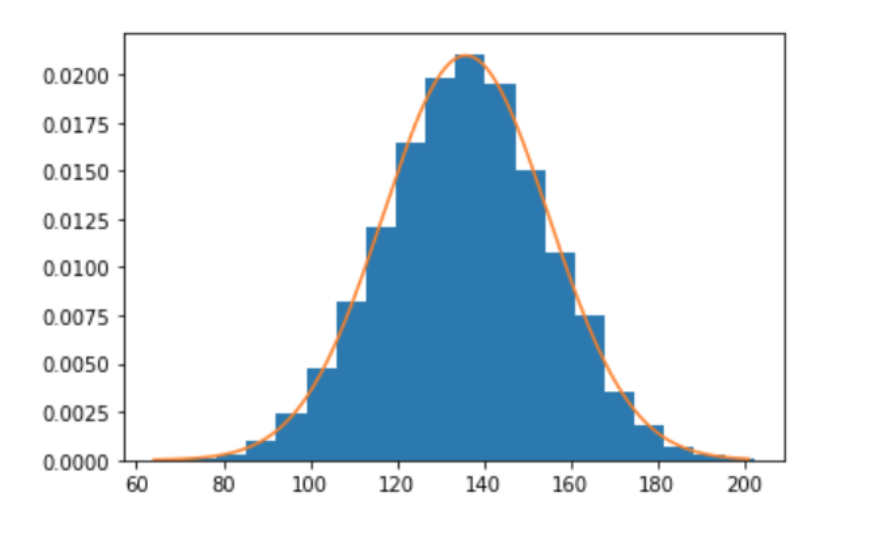
\includegraphics[width=0.4\textwidth]{figs/bins.png} }}%
	\qquad
	\subfloat[Code coverage report]{{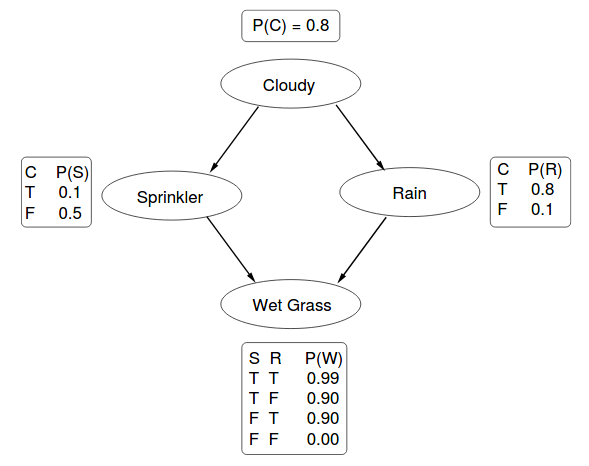
\includegraphics[width=0.4\textwidth]{figs/sprinkler-network.png} }}%
	\caption{Output from running unit tests}
	\label{fig:test-out}
\end{figure}